\appendix
%\begin{appendices}

\chapter{EPS}\label{app:EPS}
%
\section{Components Thermal Calculations}
%
\subsection*{Battery Charge Transistor}
\label{app:BCR_trans_max_heat_dissipation}
%
The worst-case power dissipation in the \ac{BCR} transistor happens when the battery is charged from its minimum charge state
%
\begin{equation}
\label{eq:BCR_trans_max_heat_dissipation}
\begin{split}
P_{transistor,max}=&(V_{in,max}-V_F-V_{bat,min})\cdot I_{charge}\\
=&(9.5\,V-0.3\,V-5.5\,V)\cdot 2.4\,A=8.88\,W
\end{split}
\end{equation}
%
where $V_{in,max}$ is the maximum mainbus voltage, $V_F$ the expected Schottky diode forward voltage drop and $V_{bat,min}$ is the preconditioning threshold voltage of the \ac{BCR} \ac{IC}. A \textit{SUP75P03-07-E3} P-channel MOSFET is selected for the \ac{BCR} charge transistor which has a maximum allowed heat dissipation of
%
\begin{equation}
P_{MOSFET,max}=\dfrac{T_J-T_A}{\theta _{JA}}=\dfrac{175\,^{\circ}C-45\,^{\circ}C}{62.5\,^{\circ}C/W}=2.08\,W
\end{equation}
%
Thus requiring a heat sink of 
%
\begin{equation}
\begin{split}
\theta_{SA} &= \frac{T_J-T_A}{P_{D,max}} - \theta_{JC} -\theta_{CS}\\ 
&=\dfrac{175^{\circ}C-45^{\circ}C}{8.88\,W}-0.8^{\circ}C/W-0.2^{\circ}C/W=13.64^{\circ}C/W
\end{split}
\end{equation}
%
%
\subsection*{Battery Charge Diode}
\label{app:BCR_diode_max_heat_dissipation}
%
A \textit{STPS20L15DPBF} Schottky diode is selected with maximum allowed heat dissipation 
%
\begin{equation}
P_{diode,max}=\dfrac{T_J-T_A}{\theta _{JA}}=\dfrac{125\,^{\circ}C-45\,^{\circ}C}{40\,^{\circ}C/W}=2\,W
\end{equation}
%
Heat dissipation in diode
%
\begin{equation}
I_{carge}V_F=2.4\,A\cdot 0.3\,V=0.72\,W
\end{equation}
%
No heat sink is required for the diode.
%
%
\section{PSpice Simulations}
\label{app:EPS_PSpice}
%
%
\begin{figure}[H]
\centering
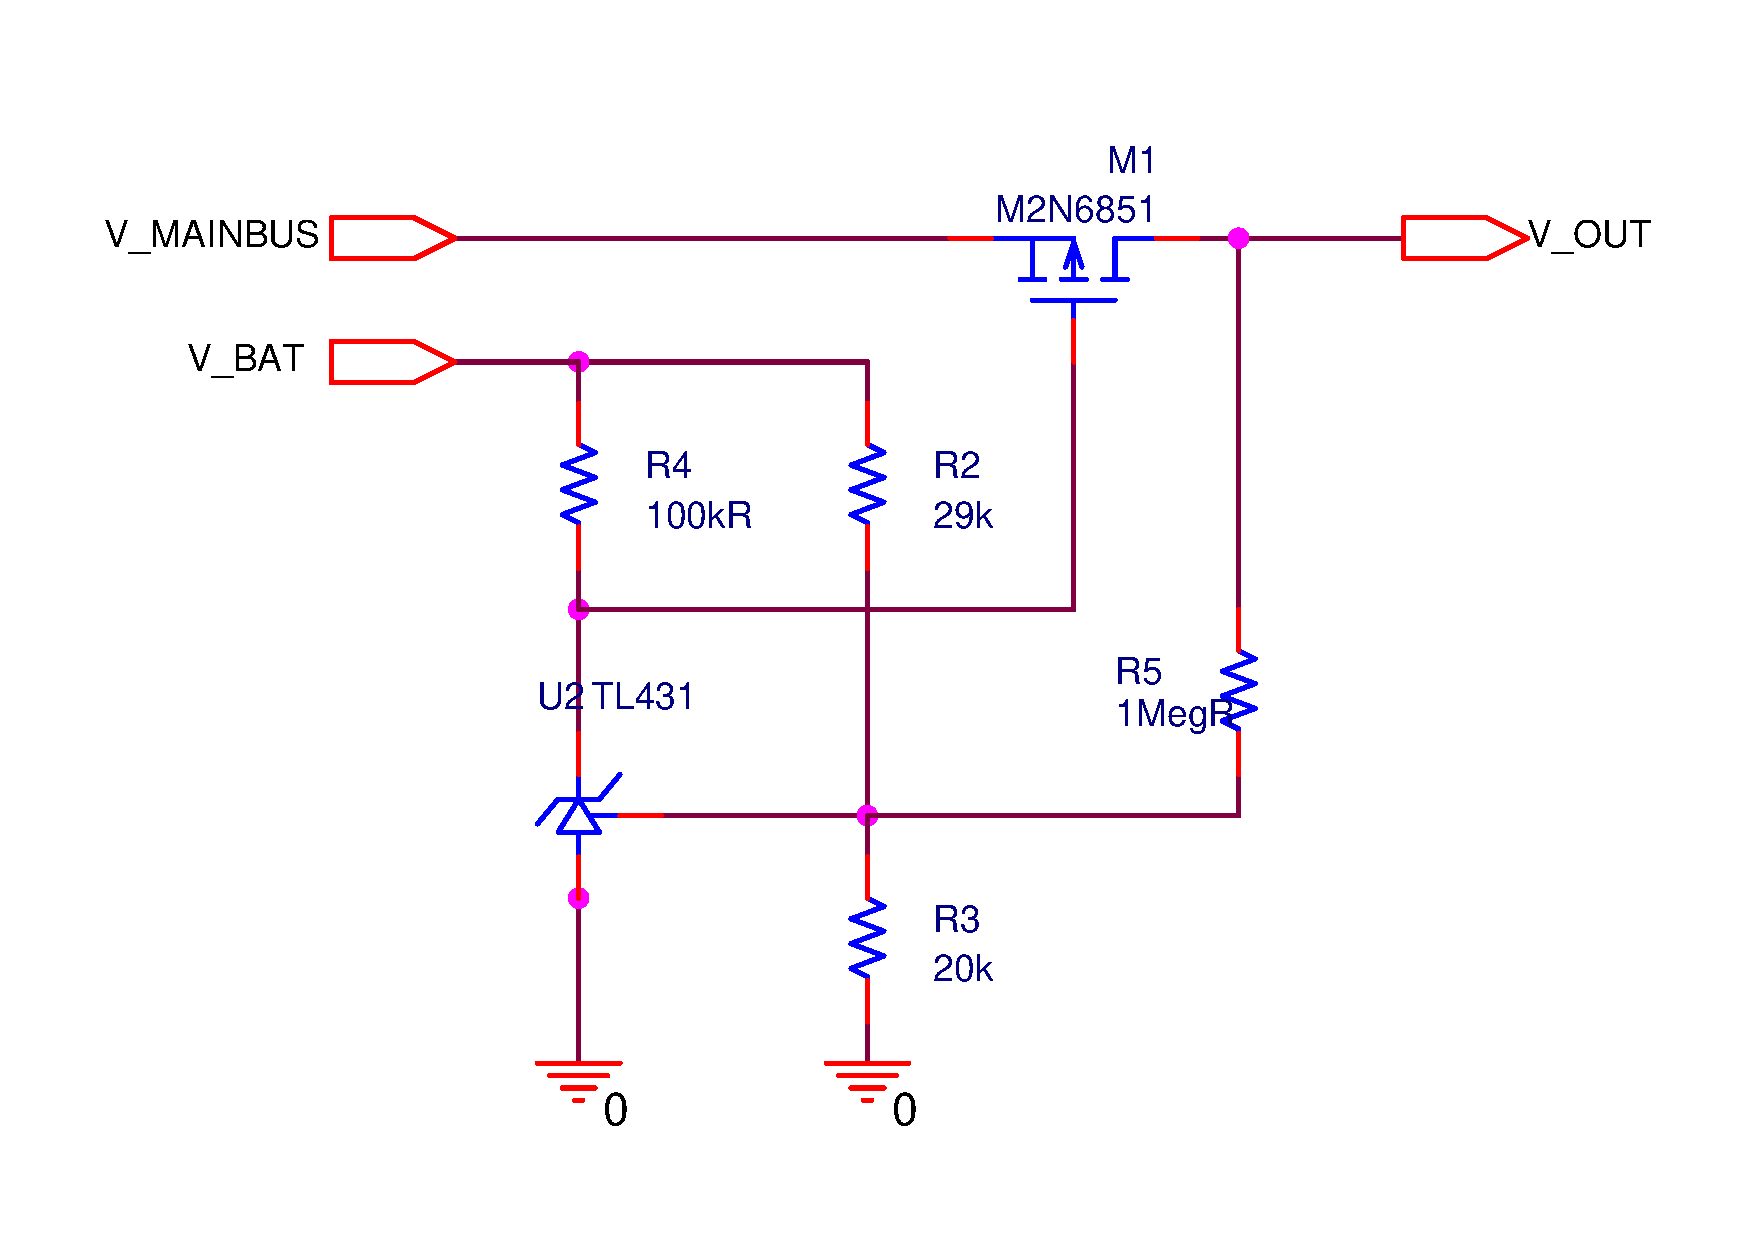
\includegraphics[scale=0.4]{figures/fig_CDR_PSpice_UVLO}
\caption{EPS UVLO circuit (PSpice)}
\label{fig:PSpice_UVLO}
\end{figure}

\begin{sidewaysfigure}
\centering
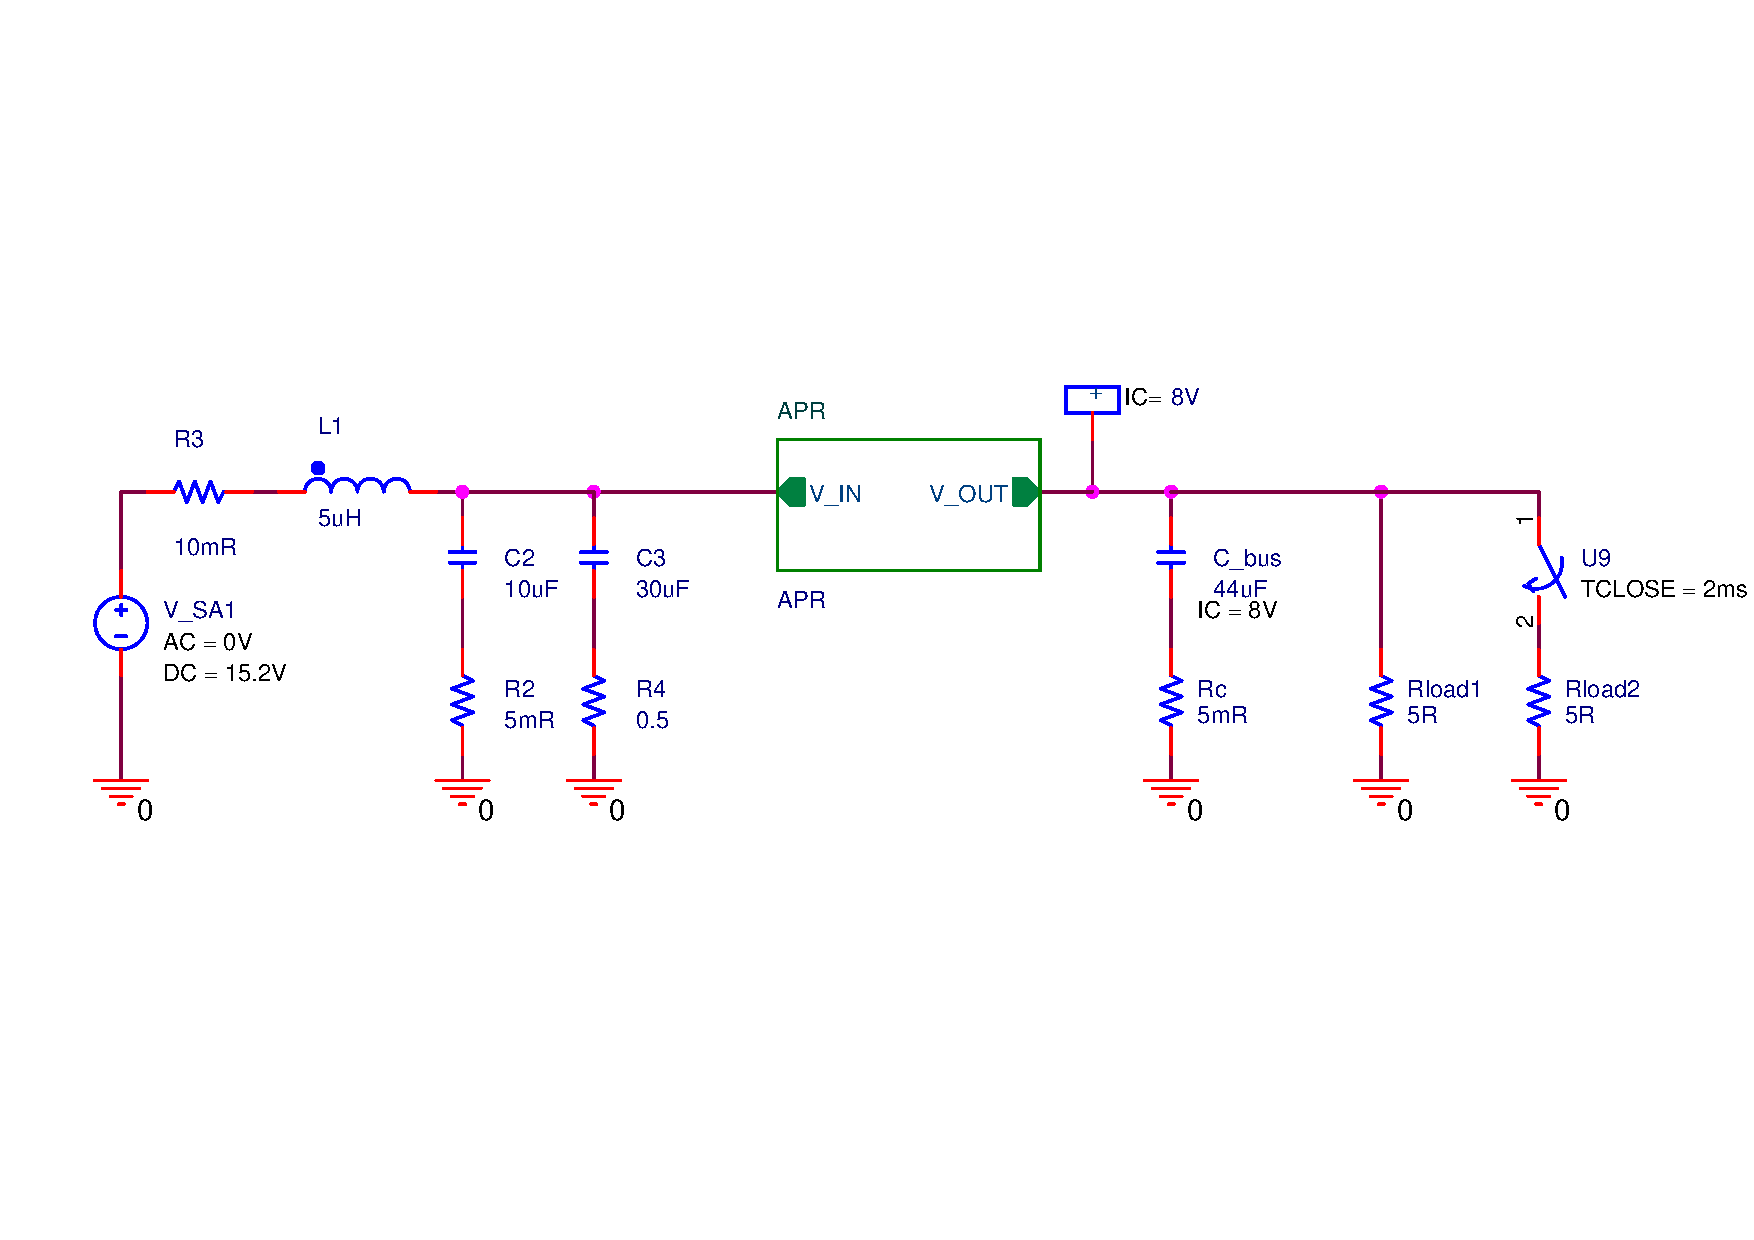
\includegraphics[scale=0.6]{figures/fig_CDR_PSpice_Mainbus}
\caption{EPS mainbus (PSpice)}
\label{fig:PSpice_mainbus}
\end{sidewaysfigure}
%
\begin{sidewaysfigure}
\centering
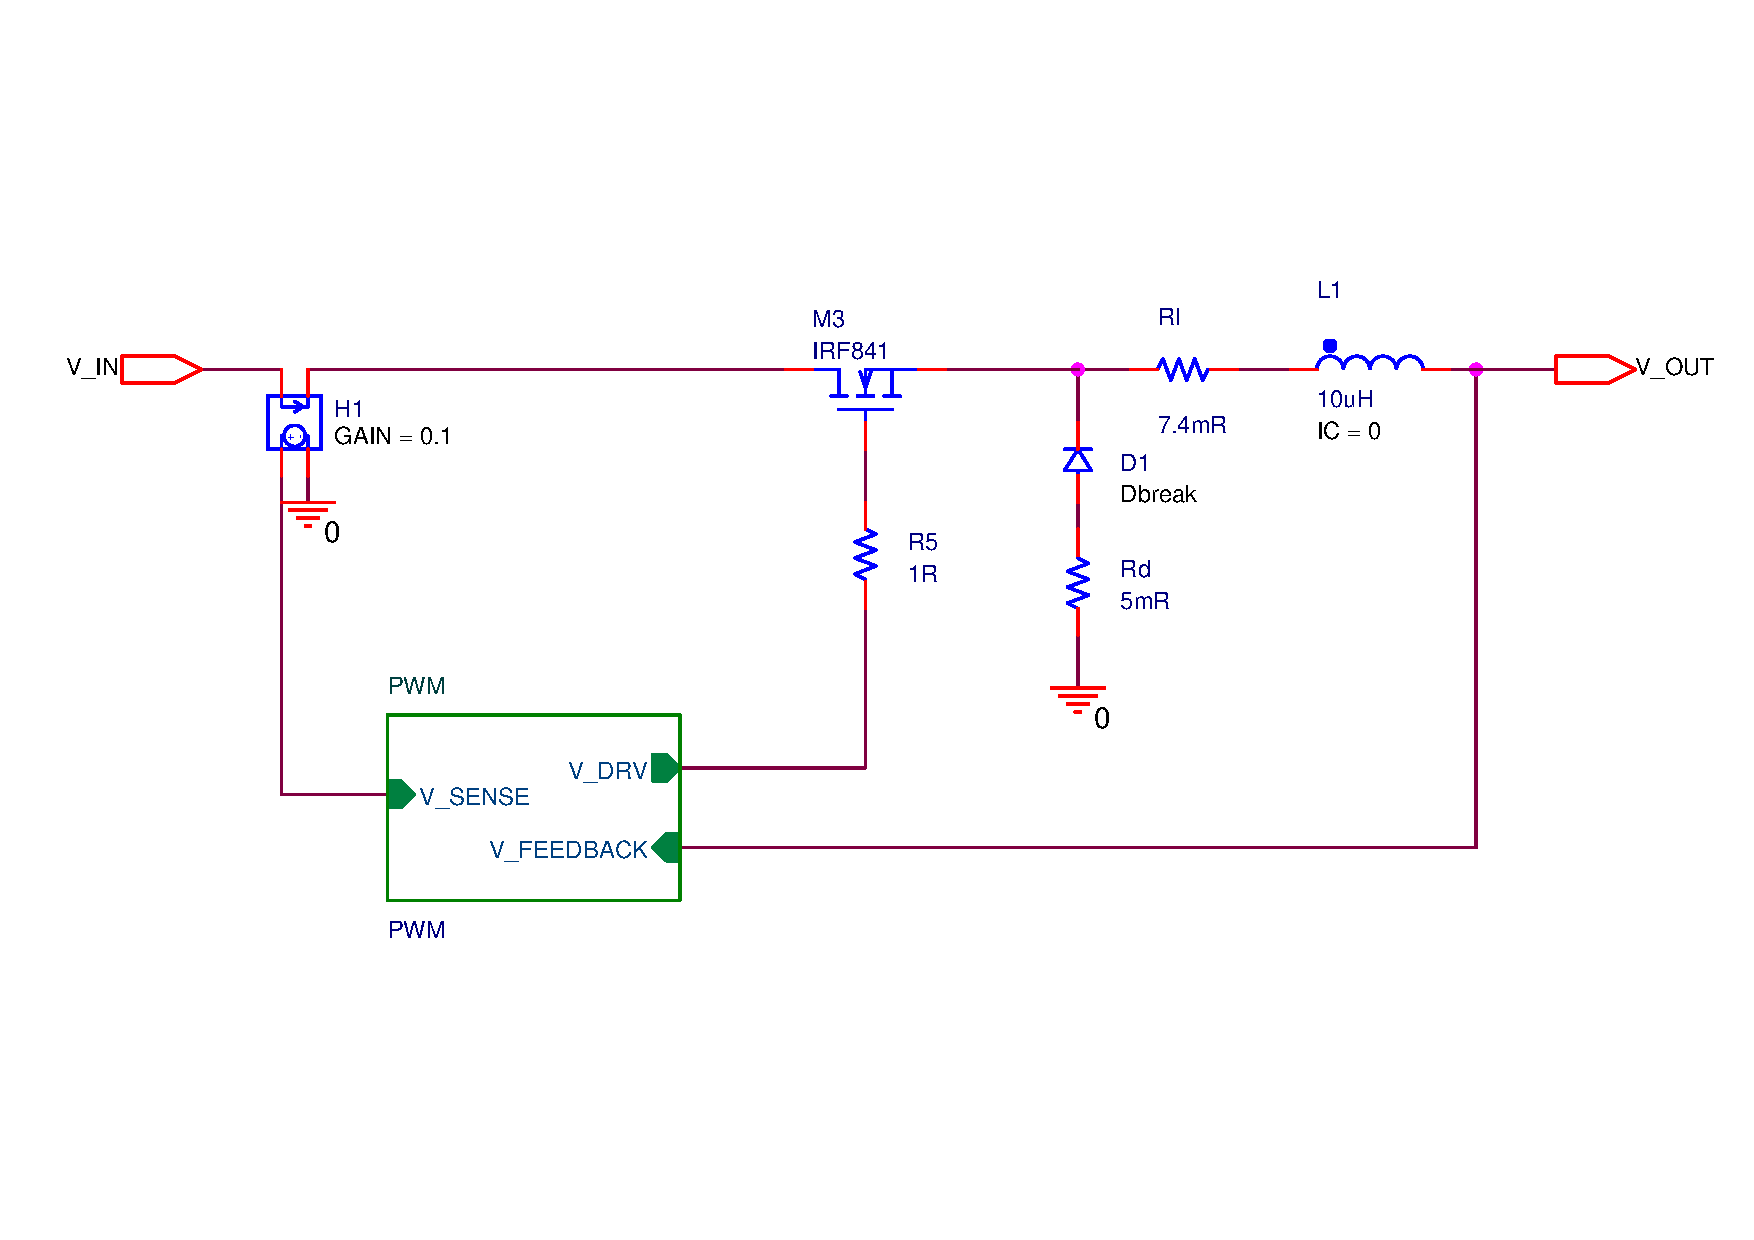
\includegraphics[scale=0.6]{figures/fig_CDR_PSpice_APR}
\caption{EPS SAR (PSpice)}
\label{fig:PSpice_SAR}
\end{sidewaysfigure}
%
\begin{sidewaysfigure}
\centering
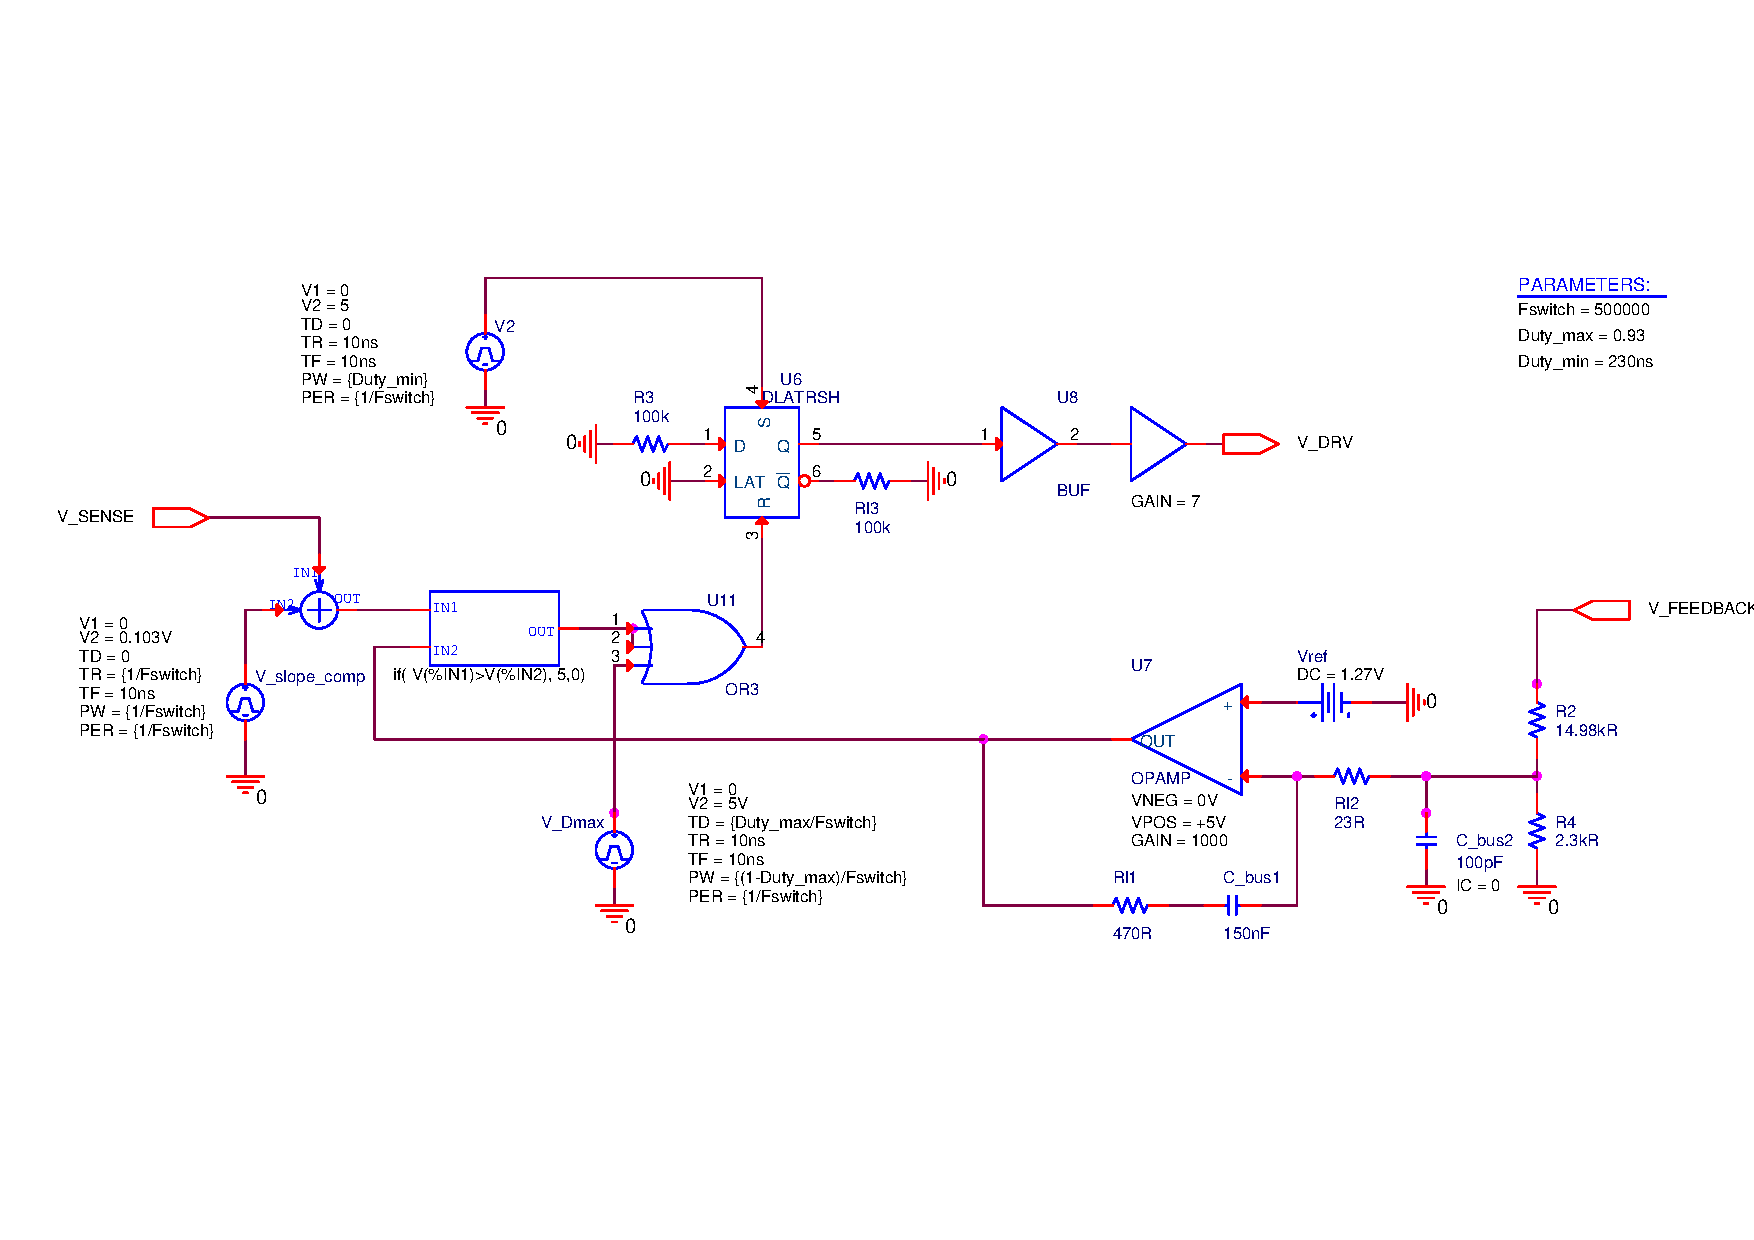
\includegraphics[scale=0.8]{figures/fig_CDR_PSpice_PWM}
\caption{EPS PWM controller (PSpice)}
\label{fig:PSpice_PWM}
\end{sidewaysfigure}
%
\newpage

\section{Mini-Mount Image}
\label{app:EPS_mini-mount}
%
\begin{figure}[h!]
\centering
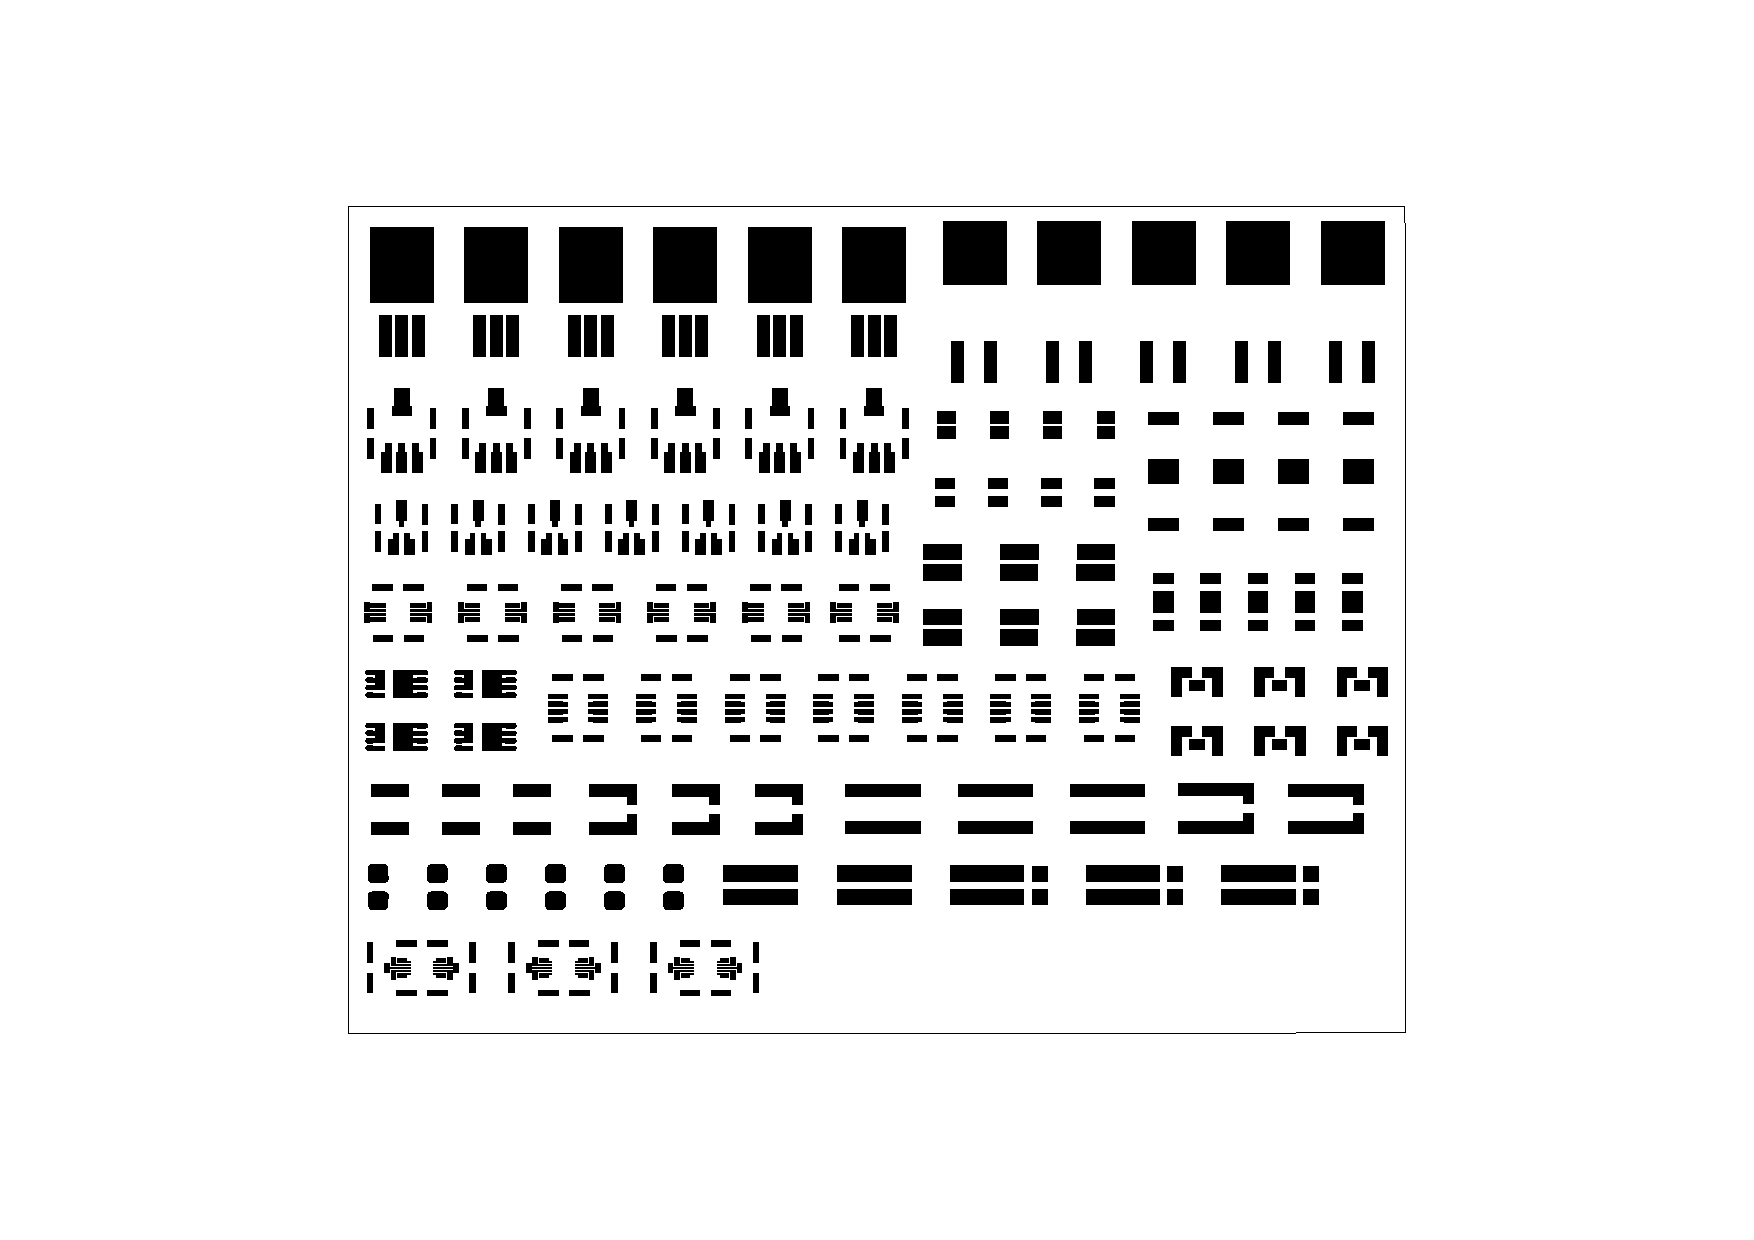
\includegraphics[scale=1,angle=90]{figures/fig_CDR_Mini-mounts}
\caption{Mini-mount prototype patches}
\label{fig:mini-mount}
\end{figure}
%
%\end{appendices}